\documentclass[crop,tikz,border=0,convert=pdf2svg,multi=false]{standalone}
\usepackage[T1]{fontenc}
\usepackage{amsfonts}
\usepackage[defaultsans]{opensans}
\usetikzlibrary{shapes,matrix,arrows,positioning}
\begin{document}
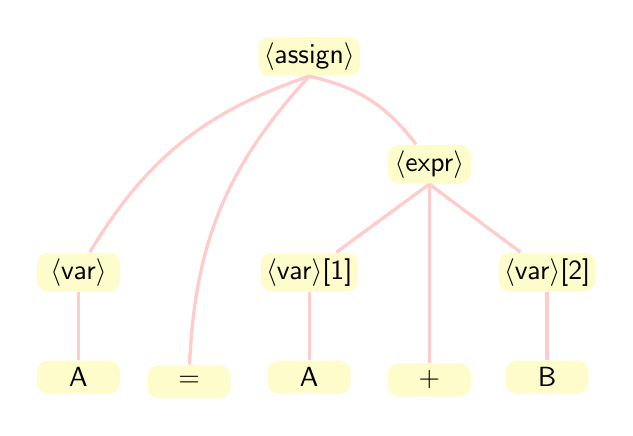
\begin{tikzpicture}[font=\sffamily,
  mymat/.style = {
    matrix of nodes, row sep=2.5em, column sep=1em, nodes=mynode},
  mynode/.style = {
    fill=yellow!20, rectangle, rounded corners, inner sep=.2em, minimum
    height=1.2em, minimum width=3em},
  edge from parent/.style=]

  \matrix (m) [mymat] {
    & & \(\langle\)assign\(\rangle\) &        & \\
    & & & \(\langle\)expr\(\rangle\) & \\
    \(\langle\)var\(\rangle\) & & \(\langle\)var\(\rangle\)[1] & & \(\langle\)var\(\rangle\)[2] \\
    A & = & A & + & B\\
  };

  \begin{scope}[red!20,very thick,draw]
    \draw (m-1-3.south) edge [bend right=20] (m-3-1);
    \draw (m-1-3.south) edge [bend right=20] (m-4-2);
    \draw (m-1-3.south) edge [bend left=20] (m-2-4);

    \draw (m-2-4.south) -- (m-3-3);
    \draw (m-2-4.south) -- (m-4-4);
    \draw (m-2-4.south) -- (m-3-5);

    \draw (m-3-1) -- (m-4-1);
    \draw (m-3-3) -- (m-4-3);
    \draw (m-3-5) -- (m-4-5);
  \end{scope}

\end{tikzpicture}
\end{document}
